\section{Conclusion}
Syntactic metathesis in Amarasi is a morphological process
used to mark the presence of a following attributive modifier.
Syntactic metathesis affects every non-final word below the level of \br{X}.
The final word of \br{X} occurs in the U\=/form,
with every previous word in the M\=/form.
A syntactic M\=/form therefore does not occur in isolation,
but canonically an typically co-occurs with a following U\=/form.


\begin{figure}[h]
	\caption{Amarasi syntactic metathesis}\label{fig:AmaSynMet}
	\centering{\Huge
		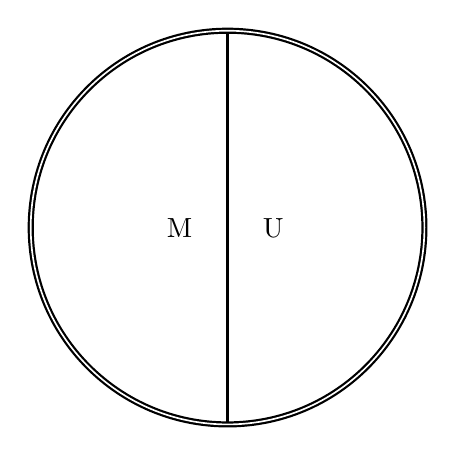
\begin{tikzpicture}[scale=.5]
			\draw[thick,double] (0,0) circle (5);
			%\draw[thick] (-5,0) -- (5,0);
			\draw[thick] (0,-4.95) -- (0,4.95);
				\node[label={[label distance=2mm]180:M}] at (0,0) {};
				\node[label={[label distance=2mm]360:U}] at (0,0) {};
		\end{tikzpicture}}
\end{figure}